\section{Discussion}
\label{section:disc}

\subsection{rcssserver}
Although rcssserver helped producing the closest thing we had to a working strategy, the general opinion regarding rcssserver is still negative. A lot of time was spent setting up basic necessities such as the UDP connection to the server, something one would think already existed as a preset for anyone to use and not have to do themselves. Not only did that take time, once that was done we had to look through the extremely limited documentation there was. The information was very vague and left a lot of things up to the readers to figure out themselves. Complications whilst running the games also appeared, as we realized we needed proper thread management to control the flow of the game which also led to time being spent solving that problem. Due to the mentioned problems, we only managed to achieve some basic training and never got to actually apply a fully finished strategy in a real game.

\subsection{Reinforcement Learning}
The results achieved by applying PPO to our VMAS RoboCup SSL setup were not as expected. Outcomes were unsatisfactory for several reasons, and further work is needed before coordinated, cooperative play can emerge.

\paragraph{Why it did not work.}
\begin{itemize}
  \item \textbf{Simulator mechanics:} Shooting and passing only worked in a very narrow pose/orientation window; small deviations often failed, so the same high-level choice produced inconsistent effects. This made the reward signal noisy and learning unstable.
  \item \textbf{Low-level skills:} High-level modes (move/dribble/shoot/pass) were mapped to hand-crafted controllers that did not always trigger predictably, so similar intents could result in weak/no kicks or unexpected ball directions.
  \item \textbf{Sparse shaping:} Rewards mostly covered progress/goals and lacked team-level signals (pass success, spacing, possession). Prior RoboCup work suggests rewarding successful, non-intercepted passes and penalising interceptions improves coordination \cite{SRC2018Team}.
  \item \textbf{Setup limits:} Minimal hyperparameter tuning, short training runs, and no role differentiation reduced stability and encouraged symmetric behaviour.
\end{itemize}

Given these issues, we did not include systematic learning curves or visualisations.

\subsection{Rule-Based System}
The success of the Rule-Based System can be attributed to its relative simplicity and deterministic nature, which enabled agents to make consistent and effective decisions. Actions were selected based on the agents' current positions on the field. While this approach may not be optimal when competing against agents powered by more advanced AI techniques, it proved highly effective against opponents that followed a predefined policy of executing the first available action. In these scenarios, the rule-based agents won every match.

\subsection{Strategy Hierarchy}
Initially, the aim was to divide the strategy into a hierarchy structure. Due to bad simulators and limited time the end product did not follow the structure that was planned from the beginning. An example of such a hierarchy is shown in figure~\ref{fig:strategy_hierarchy} and examplifies how team behavior could have been organized across 5 layers, from high-level strategy down to low-level execution. Each layer builds on the one above it, enabling modular, scalable control.  

\begin{figure}[h]
    \centering
    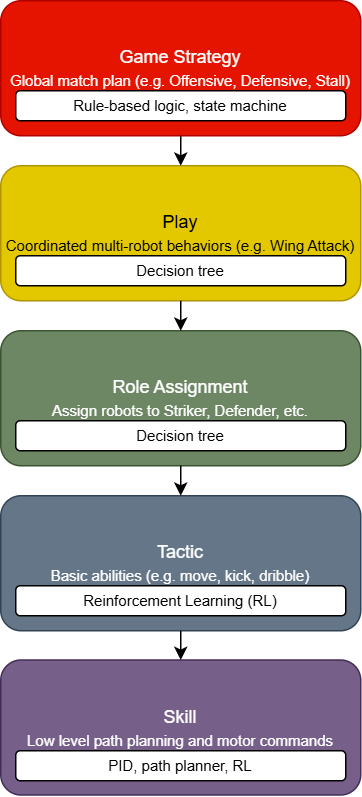
\includegraphics[width=0.8\linewidth]{./StrategyHierarchy.png}
    \caption{Hierarchical team behavior structure}
    \label{fig:strategy_hierarchy}
\end{figure}

\subsubsection{Game Strategy}
The top-layer (red box) defines the overall team behavior based on the given game state.
Then if the team is winning and the time is lower than a specified threshold, the strategy could be set to stall. This would then provide high-level context for all other decisions made below.

\subsubsection{Play}
The play layer (yellow box) could than select coordinated maneuvers such as setting up a wing attack or forming a defensive wall. Selecting plays could be done by a decision tree based on factors like ball position, team formation, and opponent layout. Each play would then set constraints or goals for roles and tactics.

\subsubsection{Role Assignment}
This layer (green box) would dynamically assign robots to specific roles (e.g. striker, defender, goalie) based on their position, proximity to the ball, or other factors.

\subsubsection{Tactic}
The tactic layer (blue box) would define what action a robot should take in its current role.
This could be whether the robot should pass, dribble, shoot, or intercept.

\subsubsection{Skill}
Lastly, the skill layer (purple box) would handle the low-level physical execution of actions.
This could be moving to a position, kicking (how hard) or dribbling. 
\vspace{1em}
Using a hierarchy like this one to structure the strategy is something that could be usefull for future works.   


For more future work, once the simulation inconsistencies are addressed, implementing more systematic evaluation of agent performance would be suitable. This would include tracking and visualizing learning curves, episode rewards, and success rates for key behaviours such as scoring and passing. These evaluation methods are necessary for diagnosing problems and refining progress on agent results.
